\documentclass[a4paper, 10pt, twocolumn, twoside]{scrartcl}
\special{papersize=210mm,297mm}
%%%%%%%%%%%%%%%%%%%%%%%%%%%%%%%%%%%%%%%%%%%%%%%%%%%%%%%%%%%%%%%%%%%%%%%%%%%%%%%
%% use the following parameter, when not using PDFLatex:                     %%
%%%%%%%%%%%%%%%%%%%%%%%%%%%%%%%%%%%%%%%%%%%%%%%%%%%%%%%%%%%%%%%%%%%%%%%%%%%%%%%
% %  dvips -t a4 ...                                                         %%
% %  ps2pdf -sPAPERSIZE=a4 ... # On Windows: ps2pdf -sPAPERSIZE#a4 ...       %%  
%%%%%%%%%%%%%%%%%%%%%%%%%%%%%%%%%%%%%%%%%%%%%%%%%%%%%%%%%%%%%%%%%%%%%%%%%%%%%%%

% uncomment or modify according to your operating system
% \usepackage[applemac]{inputenc} % european characters can be used (Mac OS)
%\usepackage[latin1]{inputenc} 
%\usepackage{fontspec}
%\usepackage{polyglossia}
\usepackage[utf8]{inputenc} % european characters can be used
\usepackage[T1]{fontenc} % hyphenation and accented letters
\usepackage{lmodern}
\usepackage{mathptmx} % times fonts
\usepackage[a4paper,twocolumn, twoside]{geometry}         
\usepackage{amsmath} % math environments, e.g. align, alignat, aligned
\usepackage{amsfonts} % additional fonts, e.g. \mathbb{}
\usepackage{amssymb} % additional math symbols
\usepackage{graphicx} % figure placement
\usepackage{tabularx}
\usepackage[usenames]{color} % color definitions
\usepackage{picture}
\usepackage{tikz} 
\usepackage{eso-pic}
\usepackage{fancyhdr} % header
\usepackage{calc}
\usepackage{hyperref}
\usepackage{ifthen}
\usepackage{forloop}
\usepackage{setspace}
\usepackage{xstring}
\usepackage[defaultsans]{opensans}
\usepackage{courier}
%\usepackage{biblatex}
%\addbibresource{references.bib}
\newcounter{startpage}

%%%%%%%%%%%%%%%%%%%%%%%%%%%%%%%%%%%%%%%%%%%%%%%%%%%%%%%%%%%%%%%%%%%%%%%%%%%%%%%%%%%%%%%%%%%%%%%%%%
%%
%% paper-specific data: to be filled out by paper-author!
%%
%%%%%%%%%%%%%%%%%%%%%%%%%%%%%%%%%%%%%%%%%%%%%%%%%%%%%%%%%%%%%%%%%%%%%%%%%%%%%%%%%%%%%%%%%%%%%%%%%%

\newcommand{\papertitle}{An open source tool for calculating \\ CO$_2$ pipeline decompression wave speed}
\newcommand{\shortpapertitle}{Open source decompression waves speed}
\newcommand{\mainauthors}{~Andreasen~ {\itshape et al.~}} % for header  
\newcommand{\authors}{Anders Andreasen\textsuperscript{1*}, N. N.\textsuperscript{1}}
\newcommand{\institutes}{
     \textsuperscript{1}Ramboll, Energy Transition, Process department, Bavneh{\o}jvej 5,
     {\color{white}\textsuperscript{1}}DK-6700 Esbjerg, Denmark; {\sffamily\itshape \textsuperscript{*}anra@ramboll.com} \\[1mm] 
     \textsuperscript{2}Bogus Institute of Applied Nonsense, 221B Metaphysics Rd, Voidshire VX04711, United Kingdom
     }
     
%% hyphenation exceptions:
\hyphenation{ Modelica }      

%%%%%%%%%%%%%%%%%%%%%%%%%%%%%%%%%%%%%%%%%%%%%%%%%%%%%%%%%%%%%%%%%%%%%%%%%%%%%%%%%%%%%%%%%%%%%%%%%%
%%%%%%%%%%%%%%%%%%%%%%%%%%%%%%%%%%%%%%%%%%%%%%%%%%%%%%%%%%%%%%%%%%%%%%%%%%%%%%%%%%%%%%%%%%%%%%%%%%

 %% use these commands to change font, fontstyle and fontsize 
%% \sfdefault ... OpenSans, \rmdefault ... Times Roman, \ttdefault ... Courier
%\usefont{T1}{\sfdefault}{bx}{n}}
%\fontsize{5cm}{1em}\selectfont 

%% set standard fonts
\renewcommand*\rmdefault{ptm}  % standard roman-font
\renewcommand*\ttdefault{pcr}  % standard type-writer-font
\renewcommand*\familydefault{\rmdefault} % default-font is roman-font

%%%%%%%%%%%%%%%%%%%%%%%%%%%%%%%%%%%%%%%%%%%%%%%%%%%%%%%%%%%%%%%%%%%%%%%%%%%%%%%%%%%%%%%%%%%%%%%%%%
%%
%% format/layout - parameter:
%%
%%%%%%%%%%%%%%%%%%%%%%%%%%%%%%%%%%%%%%%%%%%%%%%%%%%%%%%%%%%%%%%%%%%%%%%%%%%%%%%%%%%%%%%%%%%%%%%%%%
  
%\setlength{\parskip}{0.05\baselineskip}
\setlength{\parindent}{5mm}

\geometry{
     includeall,
     asymmetric, 
     bindingoffset=0mm,
     inner=21mm,
     outer = 21mm,
     nomarginpar,
     top=18.2mm,      
     headheight=4.3mm,
     headsep = 9.3mm,
     bottom=34.2mm, %30.9
     %height = 247.3mm
     footskip = 10mm,     
     columnsep=8mm,      
}

% resolution
\pdfpxdimen=1in
\divide\pdfpxdimen by 1000

%%%%%%%%%%%%%%%%%%%%%%%%%%%%%%%%%%%%%%%%%%%%%%%%%%%%%%%%%%%%%%%%%%%%%%%%%%%%%%%%%%%%%%%%%%%%%%%%%%
%%
%% custom color - definition:
%%
%%%%%%%%%%%%%%%%%%%%%%%%%%%%%%%%%%%%%%%%%%%%%%%%%%%%%%%%%%%%%%%%%%%%%%%%%%%%%%%%%%%%%%%%%%%%%%%%%%

\definecolor{SNE_DARK_BLUE}{RGB}{23, 54, 93} % used for Title
\definecolor{SNE_BLUE}{RGB}{30, 72, 124} % used section and subsection headlines, paragraph-headlines, Abstract,..
\definecolor{SNE_BRIGHT_BLUE}{RGB}{54, 94, 144} % used for header and footer
\definecolor{SNE_GRAY}{RGB}{77,77,77} % used for box with doi-number

%%%%%%%%%%%%%%%%%%%%%%%%%%%%%%%%%%%%%%%%%%%%%%%%%%%%%%%%%%%%%%%%%%%%%%%%%%%%%%%%%%%%%%%%%%%%%%%%%%
%%%%%%%%%%%%%%%%%%%%%%%%%%%%%%%%%%%%%%%%%%%%%%%%%%%%%%%%%%%%%%%%%%%%%%%%%%%%%%%%%%%%%%%%%%%%%%%%%%

\setcounter{page}{\value{startpage}}

\newcounter{ct}
\newcounter{ct2}
\newcommand{\addspaces}[1]{%
  \StrLen{#1}[\abc]
  \setcounter{ct}{\abc}
  \stepcounter{ct}
  \setcounter{ct2}{1}
  \whiledo{\value{ct} > 1}%
  {%
	\StrMid{#1}{\value{ct2}}{\value{ct2}}[\char]%
	\IfEq{\char}{ }{\hspace{1.7mm}}{\char\hspace{1.5mm}}%
	\stepcounter{ct2}%
	\setcounter{ct}{\value{ct}-1}%
   }
}

\newlength{\HSpaceLength}
\newcommand{\HSpaceOfText}[1]{\settowidth{\HSpaceLength}{#1}\hspace{\HSpaceLength}}

\makeatletter
\def\hlinewd#1{%
\noalign{\ifnum0=`}\fi\hrule \@height #1 %
\futurelet\reserved@a\@xhline}
\makeatother

%%%%%%%%%%%%%%%%%%%%%%%%%%%%%%%%%%%%%%%%%%%%%%%%%%%%%%%%%%%%%%%%%%%%%%%%%%%%%%%%%%%%%%%%%%%%%%%%%%
%%
%% configure style of headings, capture-text, ...
%%
%%%%%%%%%%%%%%%%%%%%%%%%%%%%%%%%%%%%%%%%%%%%%%%%%%%%%%%%%%%%%%%%%%%%%%%%%%%%%%%%%%%%%%%%%%%%%%%%%%

\allowdisplaybreaks[4] % page break within align-environment 0...4 priority   

\renewcommand\figurename{\footnotesize\fontsize{8.1pt}{1em}\sffamily\bfseries Figure} %% Name of figures. Change to "Abbildung" if document is written in German.
\renewcommand\tablename{\footnotesize\fontsize{8.1pt}{1em}\sffamily\bfseries Table} % Name of tables. Change to "Tabelle" if document is written in German.
\renewcommand{\refname}{\sffamily\bfseries\normalsize References}

\addtokomafont{subsection}{\color{SNE_BLUE}} %\usefont{T1}{\sfdefault}{bx}{n}}}
\addtokomafont{subsection}{\sffamily\bfseries}
\addtokomafont{subsection}{\normalsize}
\addtokomafont{section}{\sffamily\bfseries}
\addtokomafont{section}{\color{SNE_BLUE}}
\addtokomafont{section}{\Large\fontsize{14.1pt}{1em}\selectfont}
\addtokomafont{paragraph}{\sffamily\bfseries}
\addtokomafont{paragraph}{\color{SNE_BLUE}}
\addtokomafont{paragraph}{\normalsize}
\newcommand{\Abstract}[1]{\paragraph{\small\fontsize{8.7pt}{1em}\selectfont\sffamily\bfseries Abstract.}{\small\fontsize{8.7pt}{1em}\selectfont\sffamily #1}}
\newcommand{\Acknowledgement}{\section*{\color{SNE_BLUE}\sffamily\bfseries\normalsize  Acknowledgement}\vspace{-2mm}}
\newcommand{\Appendix}{\section*{\color{SNE_BLUE}\sffamily\bfseries\normalsize  Appendix}\vspace{-2mm}}
\addtokomafont{caption}{\sffamily}
\addtokomafont{caption}{\setstretch{1.3}}
\addtokomafont{caption}{\footnotesize\fontsize{8.1pt}{1.2em}\selectfont}
\addtokomafont{caption}{\raggedright}


%%%%%%%%%%%%%%%%%%%%%%%%%%%%%%%%%%%%%%%%%%%%%%%%%%%%%%%%%%%%%%%%%%%%%%%%%%%%%%%%%%%%%%%%%%%%%%%%%%
%%
%% title-section - definition:
%%
%%%%%%%%%%%%%%%%%%%%%%%%%%%%%%%%%%%%%%%%%%%%%%%%%%%%%%%%%%%%%%%%%%%%%%%%%%%%%%%%%%%%%%%%%%%%%%%%%%

\renewcommand{\maketitle}{
\twocolumn[\vspace{-3mm}{\sffamily
  {\setstretch{2.36}
    \begin{center}
      {\textcolor{SNE_DARK_BLUE}{\bfseries\huge\fontsize{19.3pt}{1em}\selectfont \papertitle}}\\
      \vspace{-0.4mm}
      {\large\fontsize{12.2pt}{1em}\selectfont \authors}
    \end{center}
  }\vspace{-0.3mm}    
  {\setstretch{1}
    {\small\fontsize{9.1pt}{1em}\selectfont \institutes }
  }}
  \vspace{7.05mm}
]
}
\setcounter{page}{1}

%%%%%%%%%%%%%%%%%%%%%%%%%%%%%%%%%%%%%%%%%%%%%%%%%%%%%%%%%%%%%%%%%%%%%%%%%%%%%%%%%%%%%%%%%%%%%%%%%%
%%%%%%%%%%%%%%%%%%%%%%%%%%%%%%%%%%%%%%%%%%%%%%%%%%%%%%%%%%%%%%%%%%%%%%%%%%%%%%%%%%%%%%%%%%%%%%%%%%


\begin{document}
\maketitle
\noindent
\parbox{\columnwidth}{
\setlength{\fboxrule}{0.8pt}
\setlength{\fboxsep}{1.7mm}
{\color{SNE_GRAY}
\fbox{
  \parbox{0.92\columnwidth}{\setstretch{1.27}\rmfamily\footnotesize\fontsize{8.1pt}{1em}\selectfont
  ~\\
  Here will be SNE-specific data positioned. \\
  To be filled out by editor. \\  
  }
}}
\setstretch{1.1}
\vspace{-1.55 mm}
\Abstract{%
%%%%%%%%%%%%%%%%%%%%%%%%%%%%%%%%%%%%%%%%%%%%%%%%%%%%%%%%%%%%%%%%%%%%%%%%%%%%%%%%%%%%%%%%%%%%%%%%%%
%% fill in abstract here:
This paper describes the calculations required to estimate the pipeline decompression velocity based on a rigorous equation of state for pure CO$_2$ and mixtures with significant impurities.
%%%%%%%%%%%%%%%%%%%%%%%%%%%%%%%%%%%%%%%%%%%%%%%%%%%%%%%%%%%%%%%%%%%%%%%%%%%%%%%%%%%%%%%%%%%%%%%%%%
}
}
\normalsize
\setstretch{1.1}
\fontsize{10.3pt}{1.15em}\selectfont
%%%%%%%%%%%%%%%%%%%%%%%%%%%%%%%%%%%%%%%%%%%%%%%%%%%%%%%%%%%%%%%%%%%%%%%%%%%%%%%%%%%%%%%%%%%%%%%%%%
%% write paper - content as usual
\section*{Introduction}

Various tools has been presented in the literature for simple calculations of the decompression wave speed such as GASDECOM \cite{Cosham_GASDECOM}, EPDECOM \cite{Lu2012_EPDECOM} and DECOM \cite{Cosham_DECOM}, which employ the assumption unidimensional isentropic, homogeneous equilibrium and inviscid formulation of the decompression wave without explicitly
solving the fluid transport equations \cite{Liu_2017}. On the other end of the scale  various 1-D/2-D CFD based tools have also been demonstrated where the mass, momentum, and energy balances are explicitly solved \cite{Xu2014_CFDDECOM,OKE20034591_pipetech_CFD,ELSHAHOMI201520_CFD}. Common to all tools is that some are purely academic and some have been developed into commercial products. However, none of the aforementioned tools are freely available to the public. In that respect, the tool presented in the present paper differentiates itself from these tools: it is open source and freely available for use by the public. 

\section{Methods}

\subsection{Decompression wave speed}
In RAMDECOM the calculation methodology for the decompression wave speed follows that shown in \cite{GU2018237,Hu2021}. When assuming the decompression wave to be isentropic, in  homogeneous equilibrium and inviscid, the decompression wave speed, $W$, is expressed as:

\begin{equation}\label{eqn:decompression}
W = C - U 
\end{equation}

where $C$ is the fluid speed of sound and $U$ is the fluid outflow velocity. The outflow velocity is given at any pressure, $P$, by:

\begin{equation}\label{eqn:outflow}
U = -\int_{P_0}^{P}{\frac{Cd\rho}{\rho}} = -\int_{P_i}^{P}{\frac{dP}{C\rho}}
\end{equation}

where $P_0$ is the initial pressure and $\rho$ is the fluid density. Integration is performed along an isentropic path. The outflow velocity in the above equation can be expressed by numerical integration using finite difference:

\begin{equation}\label{eqn:U_num}
U_i = U_{i-1} + \frac{P_{i-1}-P_i}{C_i \rho_i}
\end{equation}

where the subscript $i$ refers to the current integration step and $i-1$. Properties from the previous step is known, only density and speed of sound needs evaluation at the new step. 

In order calculate the density and the speed of sound, as well as VLE behaviour,  an adequate equation of state is required. In the currect work CoolProp \cite{coolprop} or REFPROP \cite{REFPROP} is used as the thermodynamic back-end. Both tools use Helmholtz energy formulations for fluids modelling both for pure fluids and for mixtures. For pure CO$_2$ the Span-Wagner equation of state is employed \cite{Span2009}, for mixtures the method of Lemmon \cite{Lemmon1999} and Kunz \cite{Kunz2012} is used. For mixtures with CO$_2$ the binary parameters in both CoolProp and REFPROP have been updated with those from EOS-CG \cite{Gernert2016} and later estimations by Herrig \cite{Herrig2018}. 

While the speed of sound is well defined for a single phase fluid, further assumptions are required in order to define it for two-phase / multi-phase. Assuming homogeneous equilibrium the speed of sound can generally be defined as:

\begin{equation}\label{eqn:sos}
C = \sqrt{\left( \frac{dP}{d\rho}\right)_s} \approx \sqrt{\left( \frac{P_{i-1} - P_i}{\rho_{i-1}-\rho_i}\right)}
\end{equation}

where the differential is evaluated at isentropic conditions. The full calculational workflow is the following:

\begin{itemize}
	\item Define initial conditions: $T_0$, $P_0$ and composition (either pure CO$_2$ or mixture with impurities)
	\item Calculate density and specific entropy using the equation of state
	\item For each integration step from the initial pressure the new pressure $P_i$ is set as $P_{i-1}$ + 1e5 Pa and new density is evaluated via an isentropic path.
	\begin{itemize}
		\item The speed of sound, $C_i$, is calculated via Eqn. \ref{eqn:sos} assuming a small $\Delta P$ of 100 Pa. 
		\item $C_i$ is used in Eqn.\ref{eqn:U_num} to calculate the outflow velocity $U_i$
		\item $W_i$ is calculated using Eqn. \ref{eqn:decompression}
	\end{itemize}
\end{itemize}

The calculations are generally continued until the calculated decompression wave speed becomes zero or negative. The evaluation of properties and estimation of speed of sound is performed at specified pressure and entropy (equal to the initial entropy) i.e. a PS-problem. 

For all calculations the CoolProp python wrapper is used. When using REFPROP as backend this is done still via the CoolProp wrapper. The CoolProp backend is applied only for pure CO$_2$, since the two-phase mixtures failed to solve in many cases. REFPROP can be specified both for pure CO$_2$ and for mixtures. This work is a continuation of a previous work \cite{Andreasen2021} with the purpose of building useful engineering tools on top of high quality open source software packages. RAMDECOM is developed entirely in python 3 and also relies on other python packages such as pandas \cite{mckinney-proc-scipy-2010}, matplotlib \cite{Hunter:2007}, and numpy \cite{harris2020array}. 

\subsection{Experimental}
In order to compare the presented decompression model with experimental data various relevant experiments have been sourced from the literature. For decompression of pure CO$_2$ experiments made by Munkejord \emph{et al.} \cite{MUNKEJORD2020118560} and Botros \emph{et al.} \cite{Botros_pure}. For CO$_2$ rich mixtures the experiments from Botros \emph{et al.} \cite{Botros_mixture} has been sourced. 

All the experiments sourced have similar set-up and many things in common. The experiments are performed in a horizontal shock-tube comprised of a number of tubular sections flanged together and equipped with pressure and temperature transducers located along the length of the shock-tube. One end is closed and the other end is equipped with a rupture disc. In order to ensure controllable and uniform temperature the shock-tube is heat traced and insulated. The facilities has mixing and compression units in order to fill the shock tube with the desired mixture and the desired initial pressure. For additional information about experimental methods and facility description and details please refer to the original papers \cite{MUNKEJORD2020118560,Botros_pure}.

The experimental test conditions for the pure CO$_2$ experiments are summarised in Table \ref{tbl:pure_exp} and the experimental test conditions for the CO$_2$ rich mixtures are summarised in Table \ref{tbl:mix_exp}.

\begin{table}[h]
	\renewcommand{\arraystretch}{1.3}
	\centering
	\begin{tabularx}{\columnwidth}{l|l|l|X}\hlinewd{1.2pt}

\textbf{Exp No.} & \textbf{P (bar)}	&	\textbf{T ($^\circ$C)} 	& \textbf{Source} \\ \hlinewd{1pt}
3		& 40.4		&	10.2	& Munkejord et al.\\
6		& 104		&	40		& Munkejord et al. \\
8		& 122.2		&	24.6	& Munkejord et al. \\
15		& 340.4		&	36.5	& Botros et al. \\
31		& 111.11	&	35.04	& Botros et al. \\
32A		& 112.7		&	8.74	& Botros et al. \\ \hlinewd{1.2pt}
	\end{tabularx}
\caption{Experimental initial conditions for decompression experiments with pure CO$_2$ from Munkejord \emph{et al.} \cite{MUNKEJORD2020118560} and Botros \emph{et al.} \cite{Botros_pure}.}
\label{tbl:pure_exp}
\end{table}

\begin{table*}[!h]
	\renewcommand{\arraystretch}{1.3}
	\centering
	\begin{tabularx}{\textwidth}{l|l|l|l|l|l|l|l|l|l|l}\hlinewd{1.2pt}
				& & & \multicolumn{8}{c}{\textbf{Composition (mole \%)}} \\ \hlinewd{1pt}
		\textbf{Exp No.} & \textbf{Pressure (bar)}	&	\textbf{Temperature ($^\circ$C)} 	& \textbf{CO$_2$} & \textbf{N$_2$} & \textbf{O$_2$} & \textbf{He} & \textbf{Ar} & \textbf{CO} & \textbf{H$_2$} & \textbf{CH$_4$} \\ \hlinewd{1pt}

2	&	148.3	& 35.9 & 94.03  & 5.82  & 0.127 & 0.025 & 		& 		&      & 	 \\				
4	&	145.6	& 35.1 & 96.67 	& 		& 3.33  & 		& 		& 		& 	   & 	 \\			
7	&   147.8	& 36.3 & 96.52  & 		& 		& 0.0138& 		& 		& 	   & 3.47\\
10B	&	149.3	& 35.3 & 96.77  & 		& 		& 		& 		& 		& 3.23 & 	 \\	
5	&   144.9	& 35.6 & 96.77  & 0.0025& 		& 		& 		& 3.23	& 	   & 	 \\		
9	&   154.6	& 35.2 & 96.14  & 		& 		& 		& 3.86 	& 		& 	   &	 \\ \hlinewd{1.2pt}			
	\end{tabularx}
	\caption{Experimental initial conditions for decompression experiments with pure CO$_2$ from  Botros \emph{et al.} \cite{Botros_mixture}.}
	\label{tbl:mix_exp}
\end{table*}

\section{Results and discussion}
\subsection{Pure CO$_2$}
The experiments for pure CO$_2$ summarised in Table \ref{tbl:pure_exp} have all been simulated using the Span \& Wagner equation of state as provided by CoolProp. The isentropic decompression path for all simulated cases is shown in Figure \ref{fig:pure_envelope}.The path from the inital pressure and temperature in the single phase region to the saturation line. The experimental initial conditions cover both gas, liquid (supercritical), and supercritical fluid. Once the decompression state reaches the saturation line the isentrope follows the saturation line with varying fase split. Calculations have been done with the REFPROP backend as well, and identical results where obtained (not shown).  

\begin{figure}[!ht]
\centering
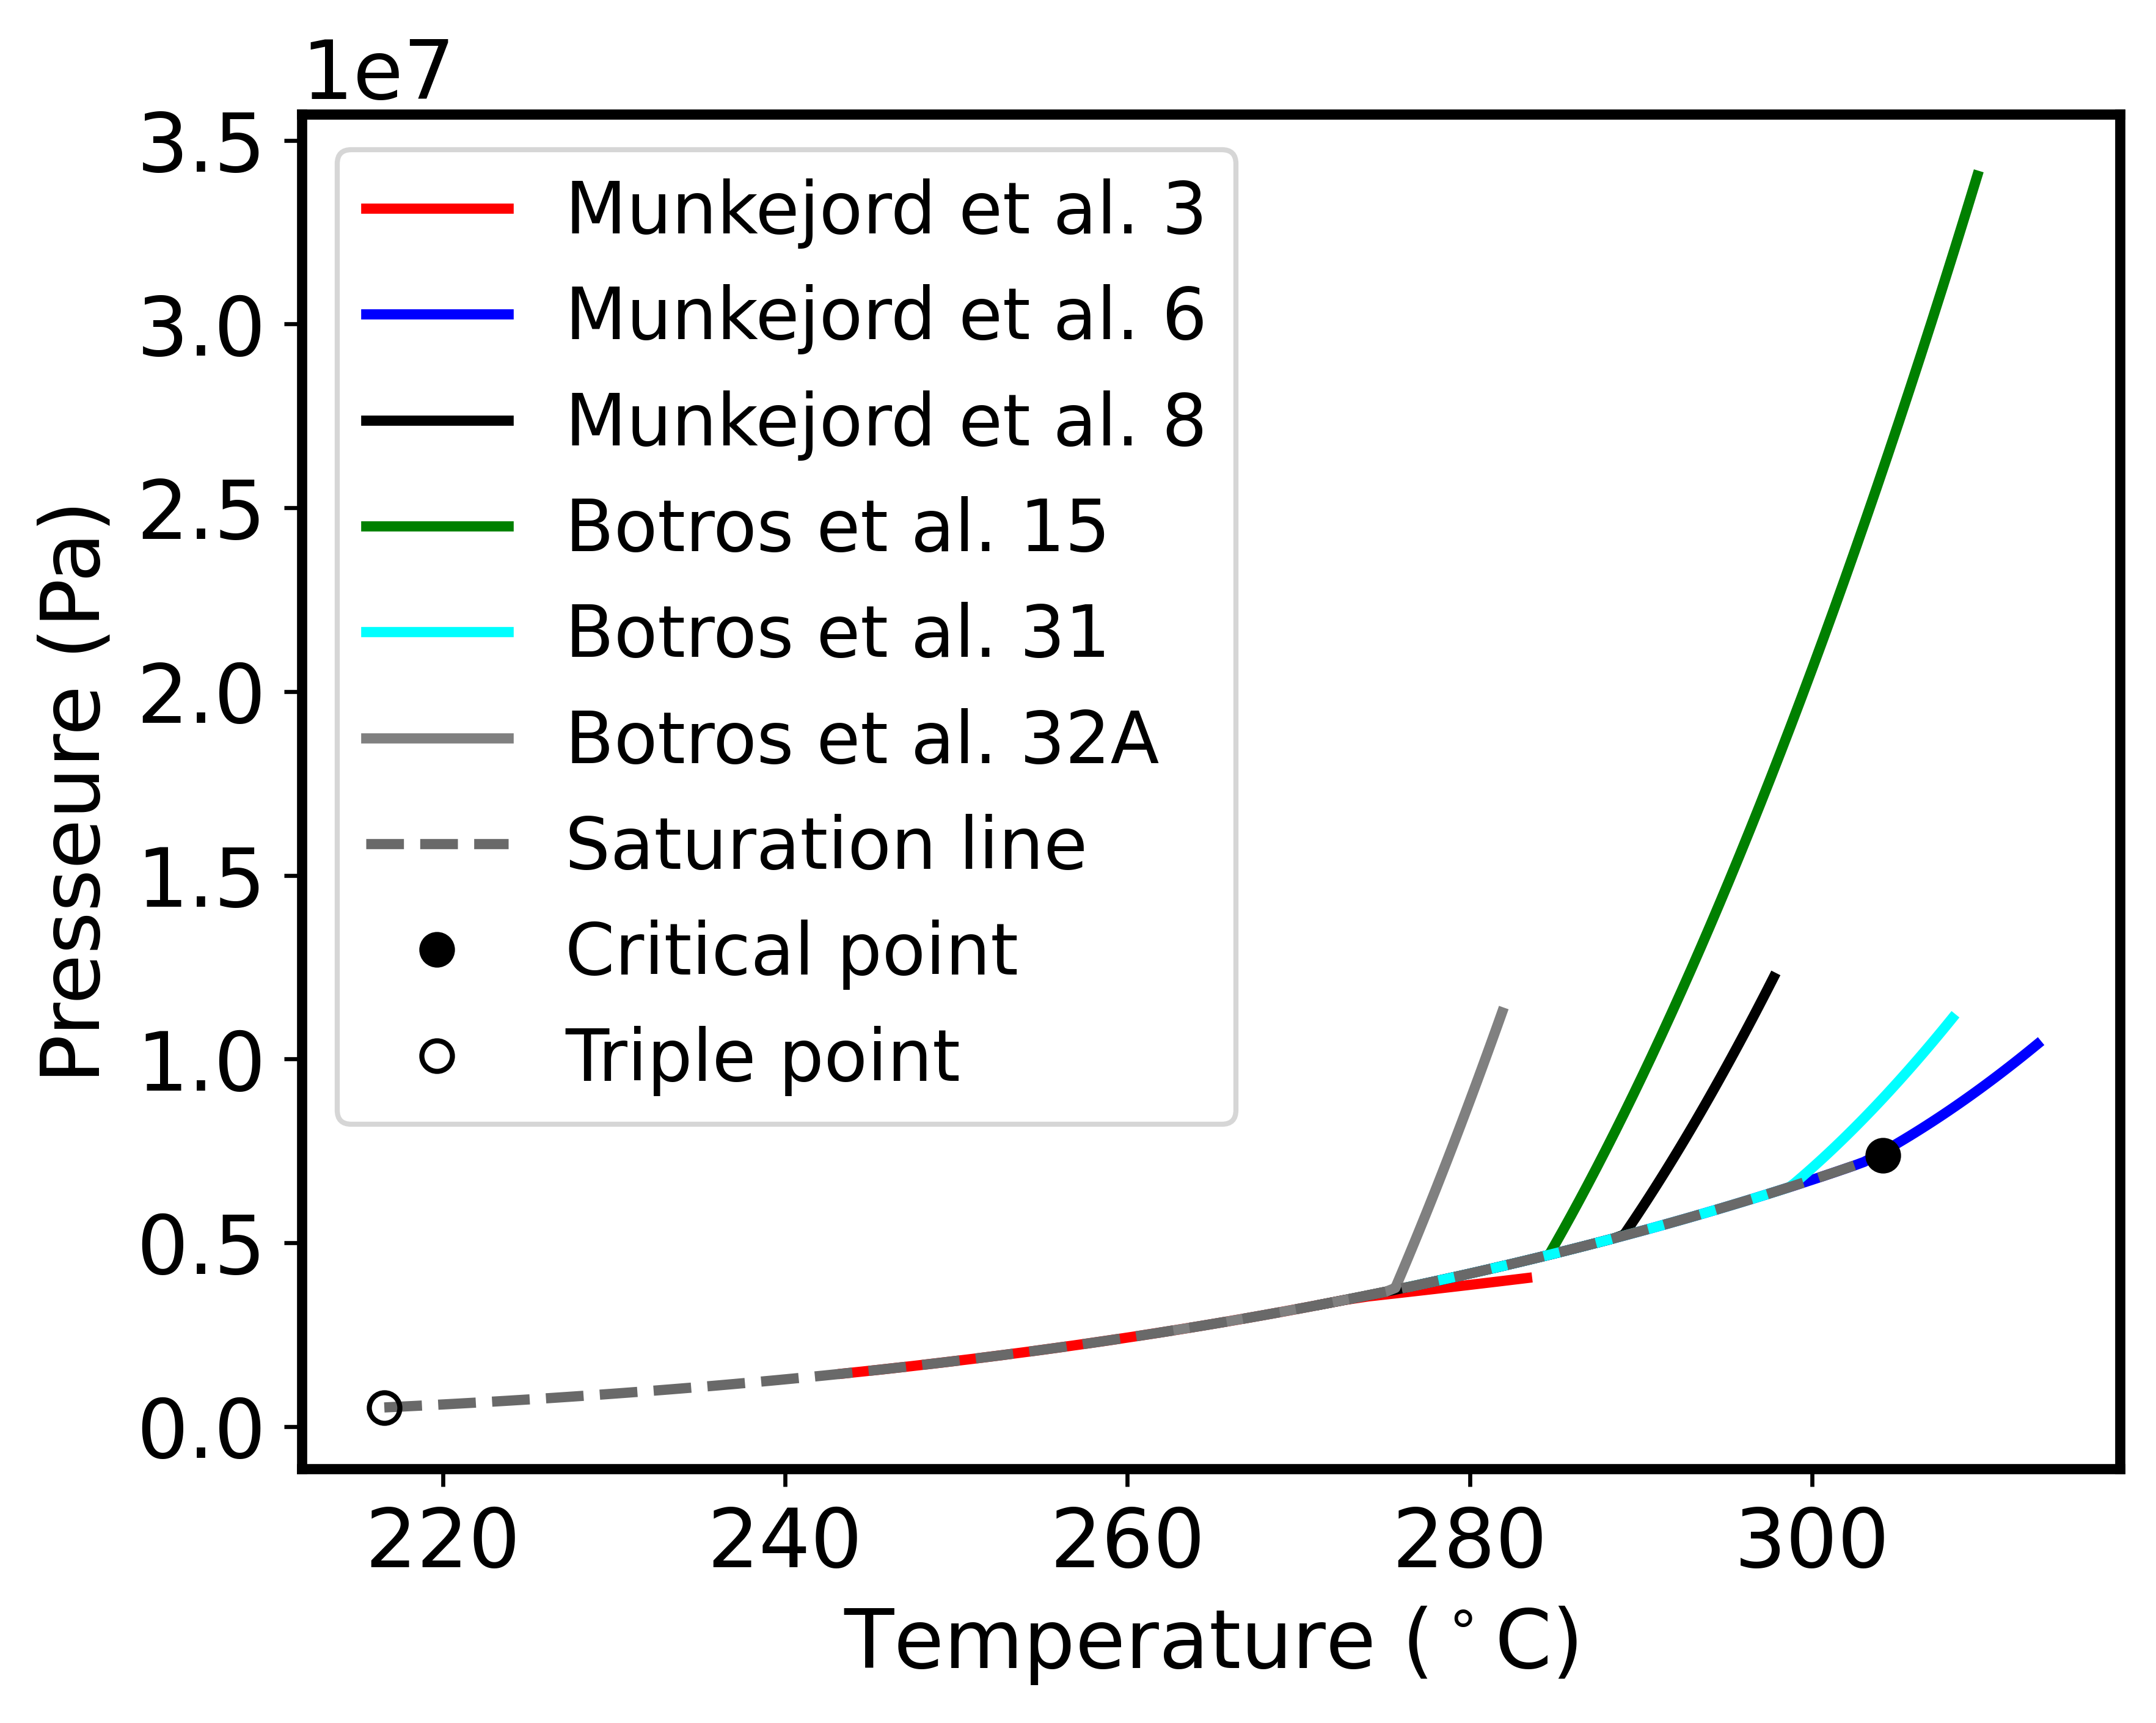
\includegraphics[width=\columnwidth]{./Bilder/pure_envelope.png}
\caption{Isentropic decompresion path for all simulated cases for pure CO$_2$ shown in the P,T plane along with the saturation curve for pure CO$_2$ from triple point to the critical point. }
\label{fig:pure_envelope}
\end{figure}

Decompression wave speed plots are made for all cases and corresponding experimental data has been sourced from \cite{MUNKEJORD2020118560,Botros_pure}. It shall be noted that the experimental points have been read manually with the aid of the ScanIT program from Amsterchem \footnote{\url{https://www.amsterchem.com/scanit.html}}. Some slight inaccuracy during the digitization of data from the original references must be expected and further in some areas the original data was too dense to allow all data points to be extracted. That being said the overall characteristics and the shape of the decompression curves have been retained. 

The decompression curves for experiments 6 and 8 from \cite{MUNKEJORD2020118560} and experiments 31 and 32A from \cite{Botros_pure} are grouped in the same plot cf. Figure \ref{fig:pure_combined} whereas experiments 3 from \cite{MUNKEJORD2020118560} and 15 from \cite{Botros_pure} are plotted individually in Figures \ref{fig:pure_3} and \ref{fig:pure_15} , respectively.
 
\begin{figure}[!ht]
	\centering
	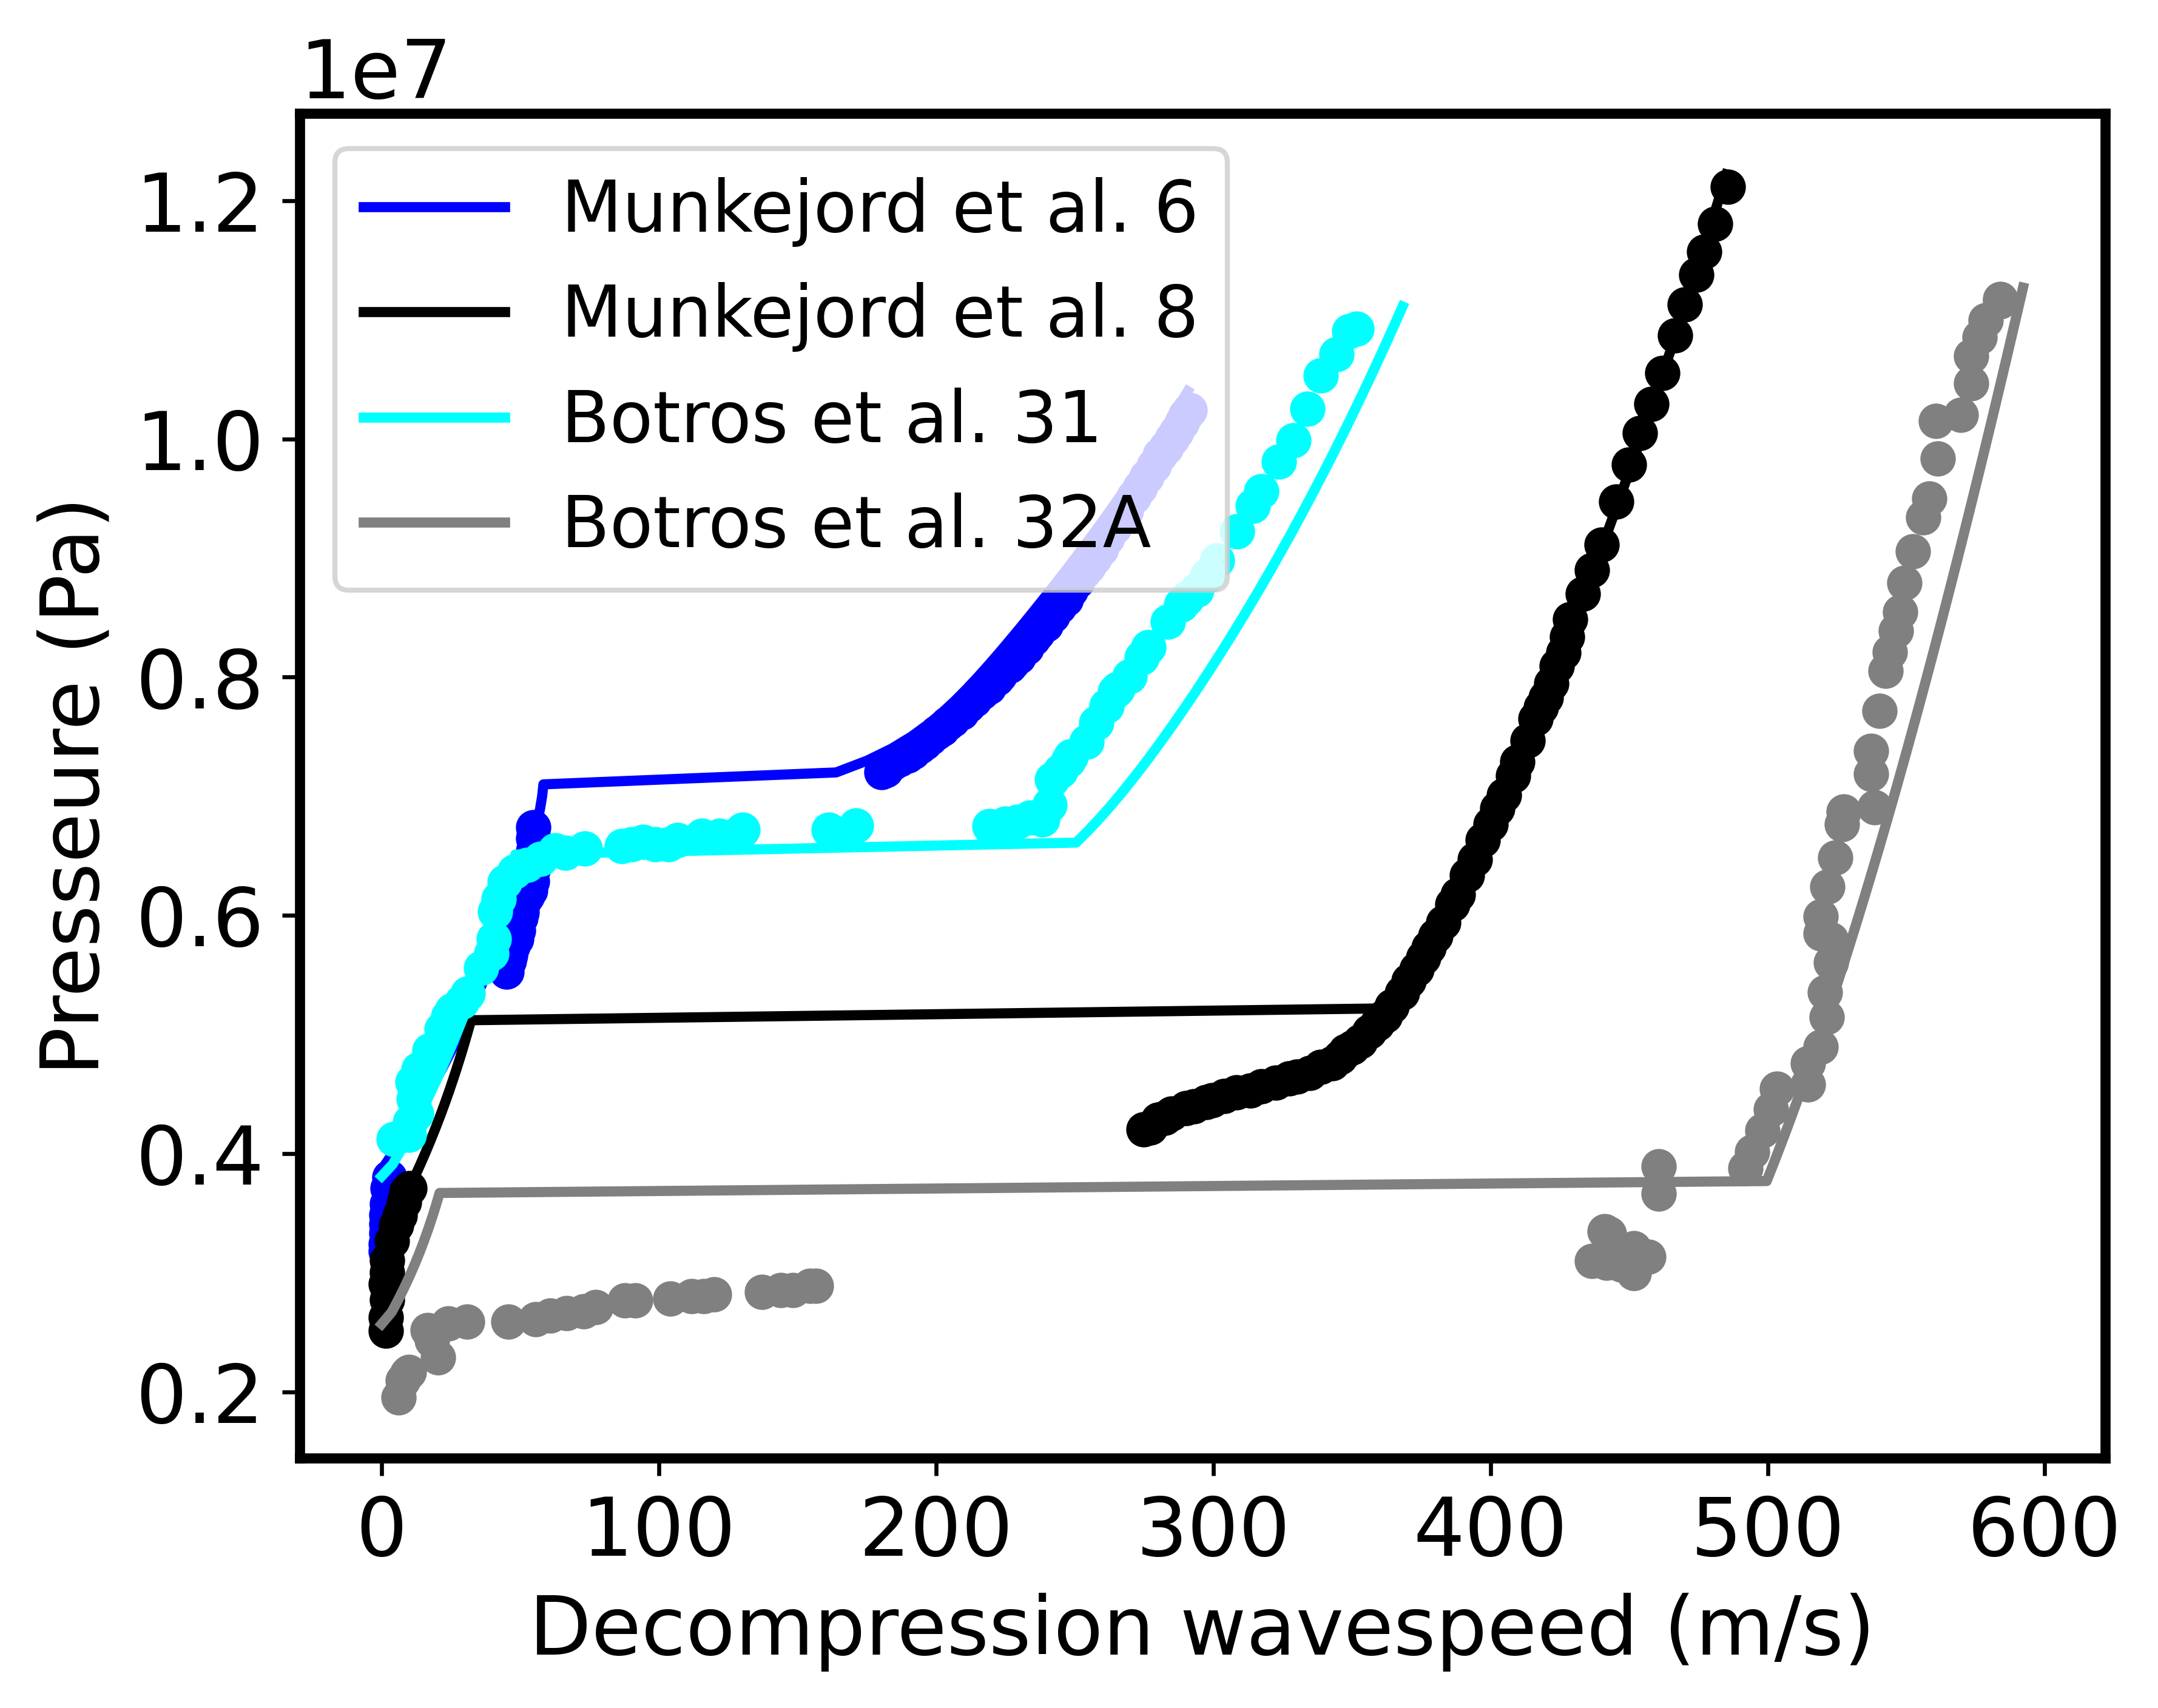
\includegraphics[width=\columnwidth]{./Bilder/pure_combined.png}
	\caption{Decompression curves for pure CO$_2$ calculated with the RAMDECOM code and experimental data.}
	\label{fig:pure_combined}
\end{figure}

\begin{figure}[!ht]
	\centering
	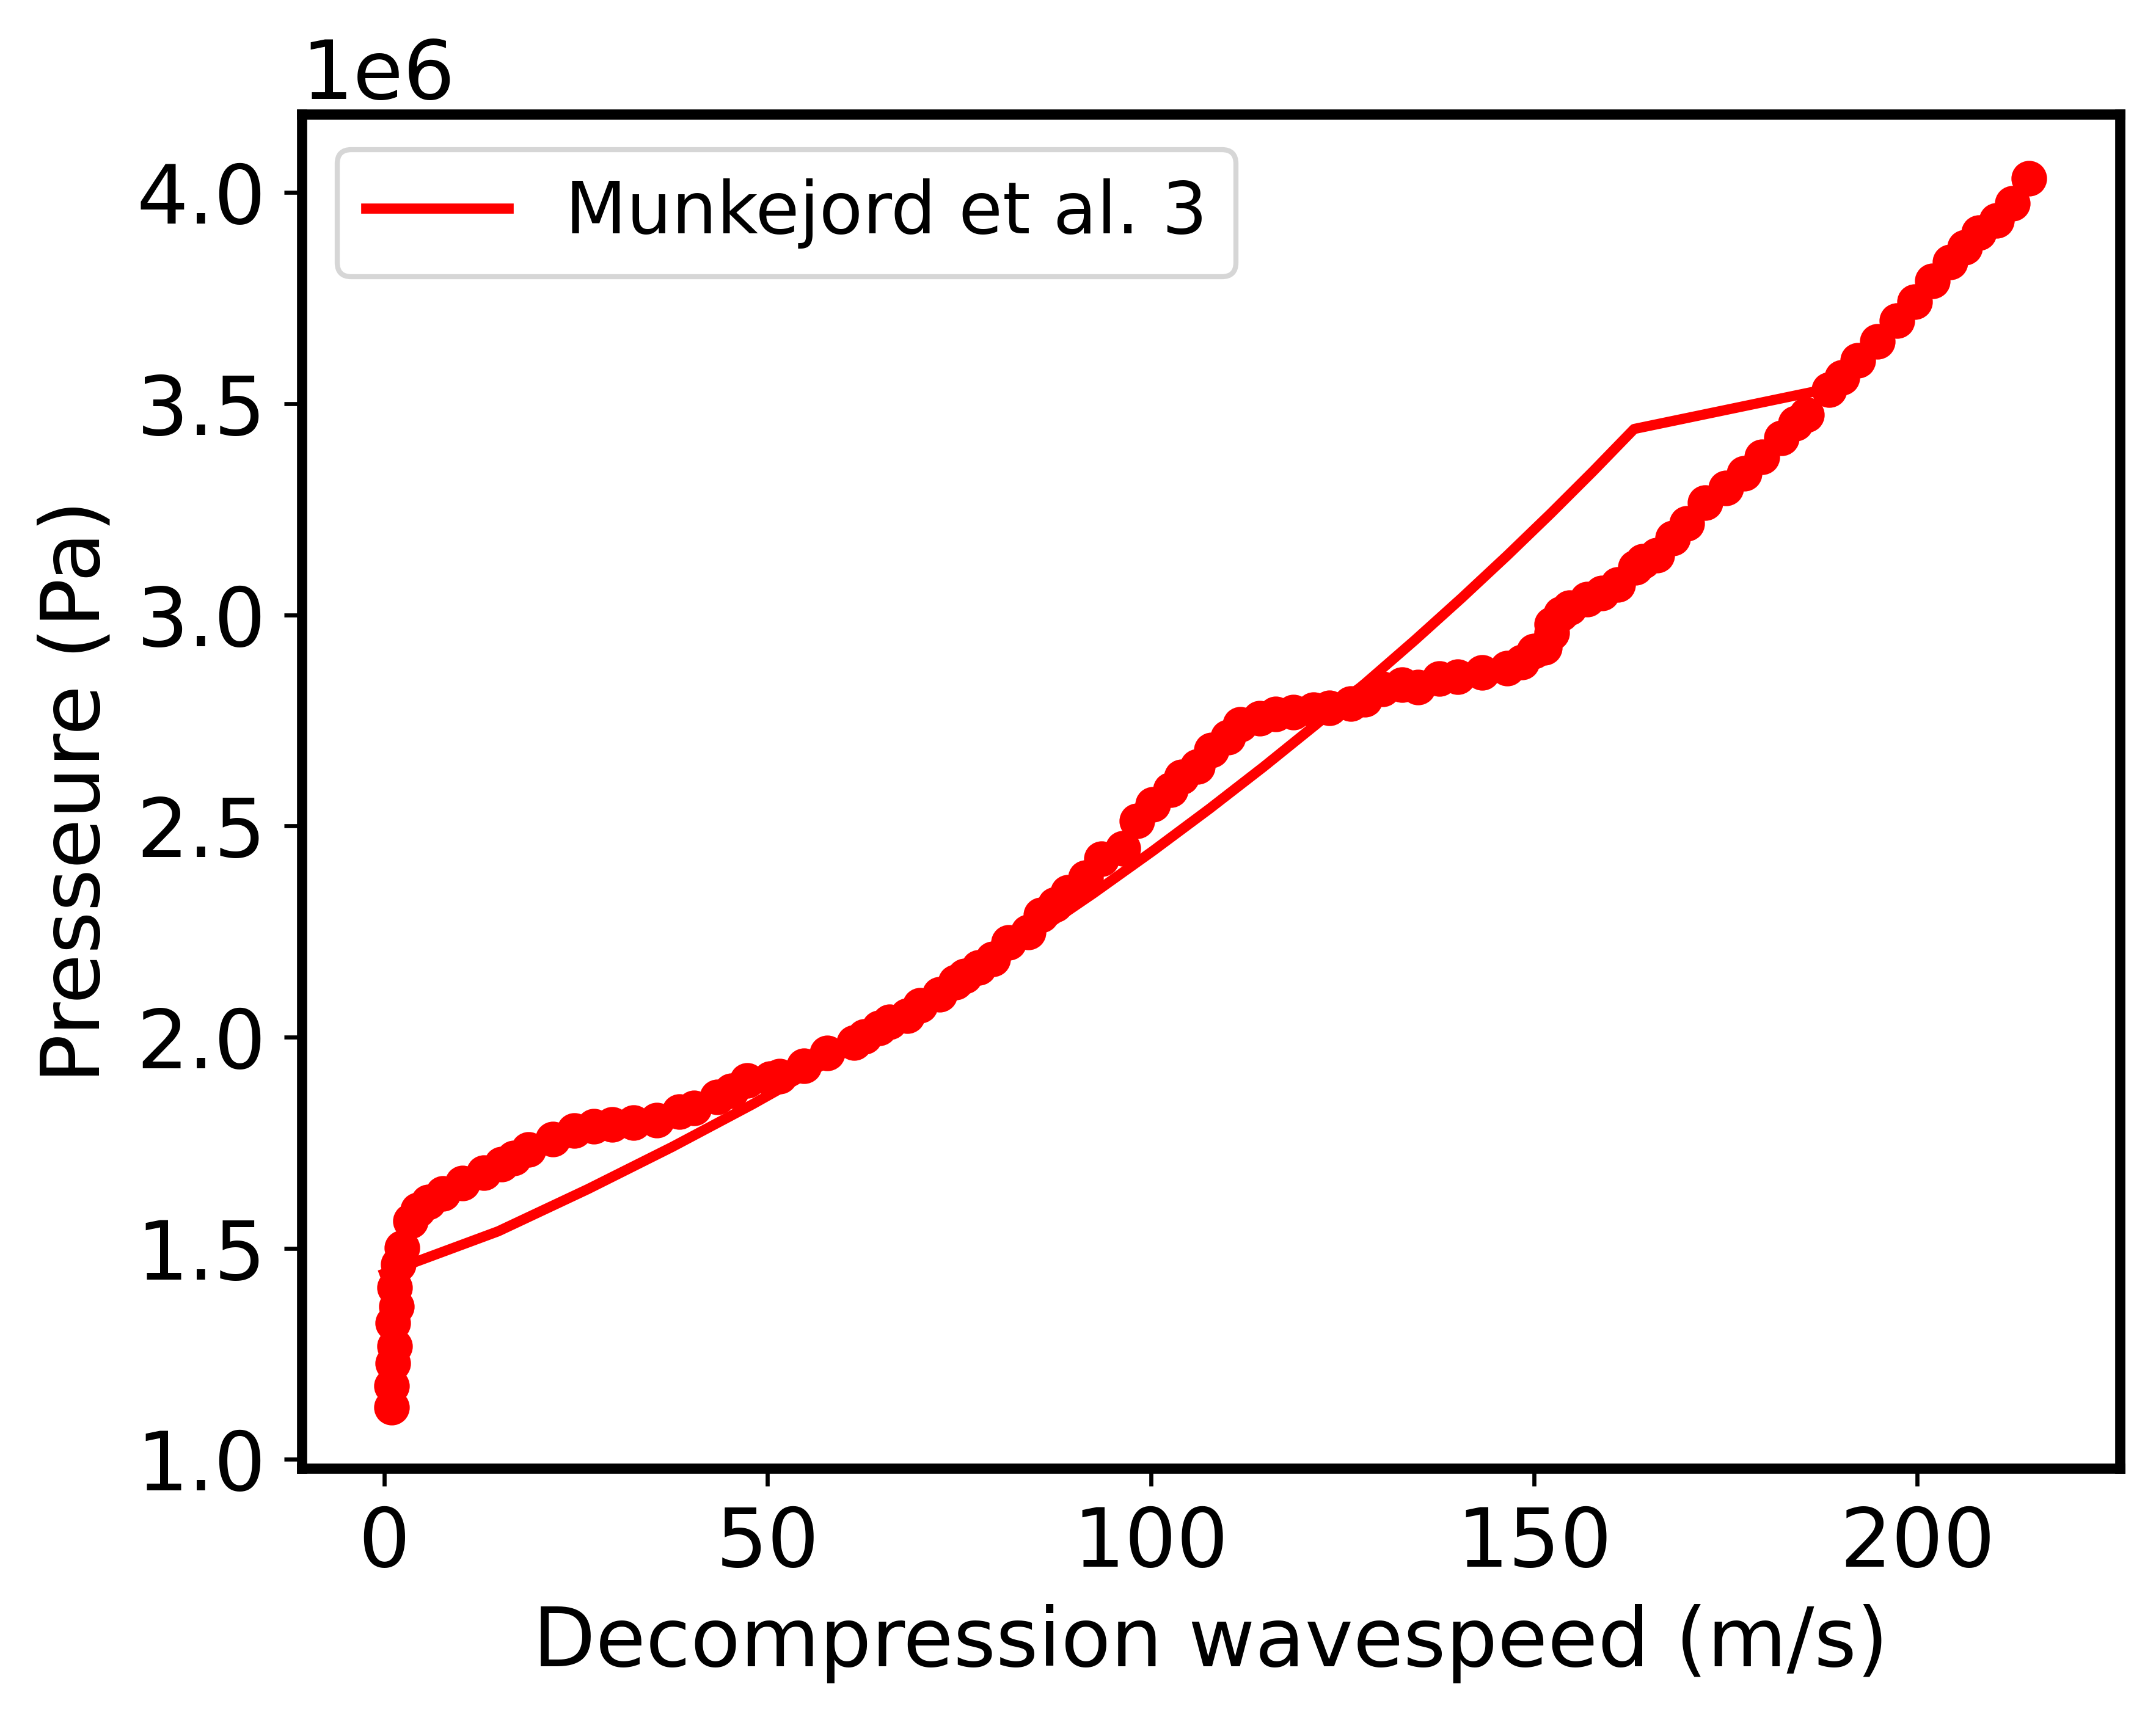
\includegraphics[width=\columnwidth]{./Bilder/pure_0.png}
	\caption{Decompression curve for pure CO$_2$  calculated with the RAMDECOM code and data for experiment 3 from \cite{MUNKEJORD2020118560}.}
	\label{fig:pure_3}
\end{figure}

\begin{figure}[!ht]
	\centering
	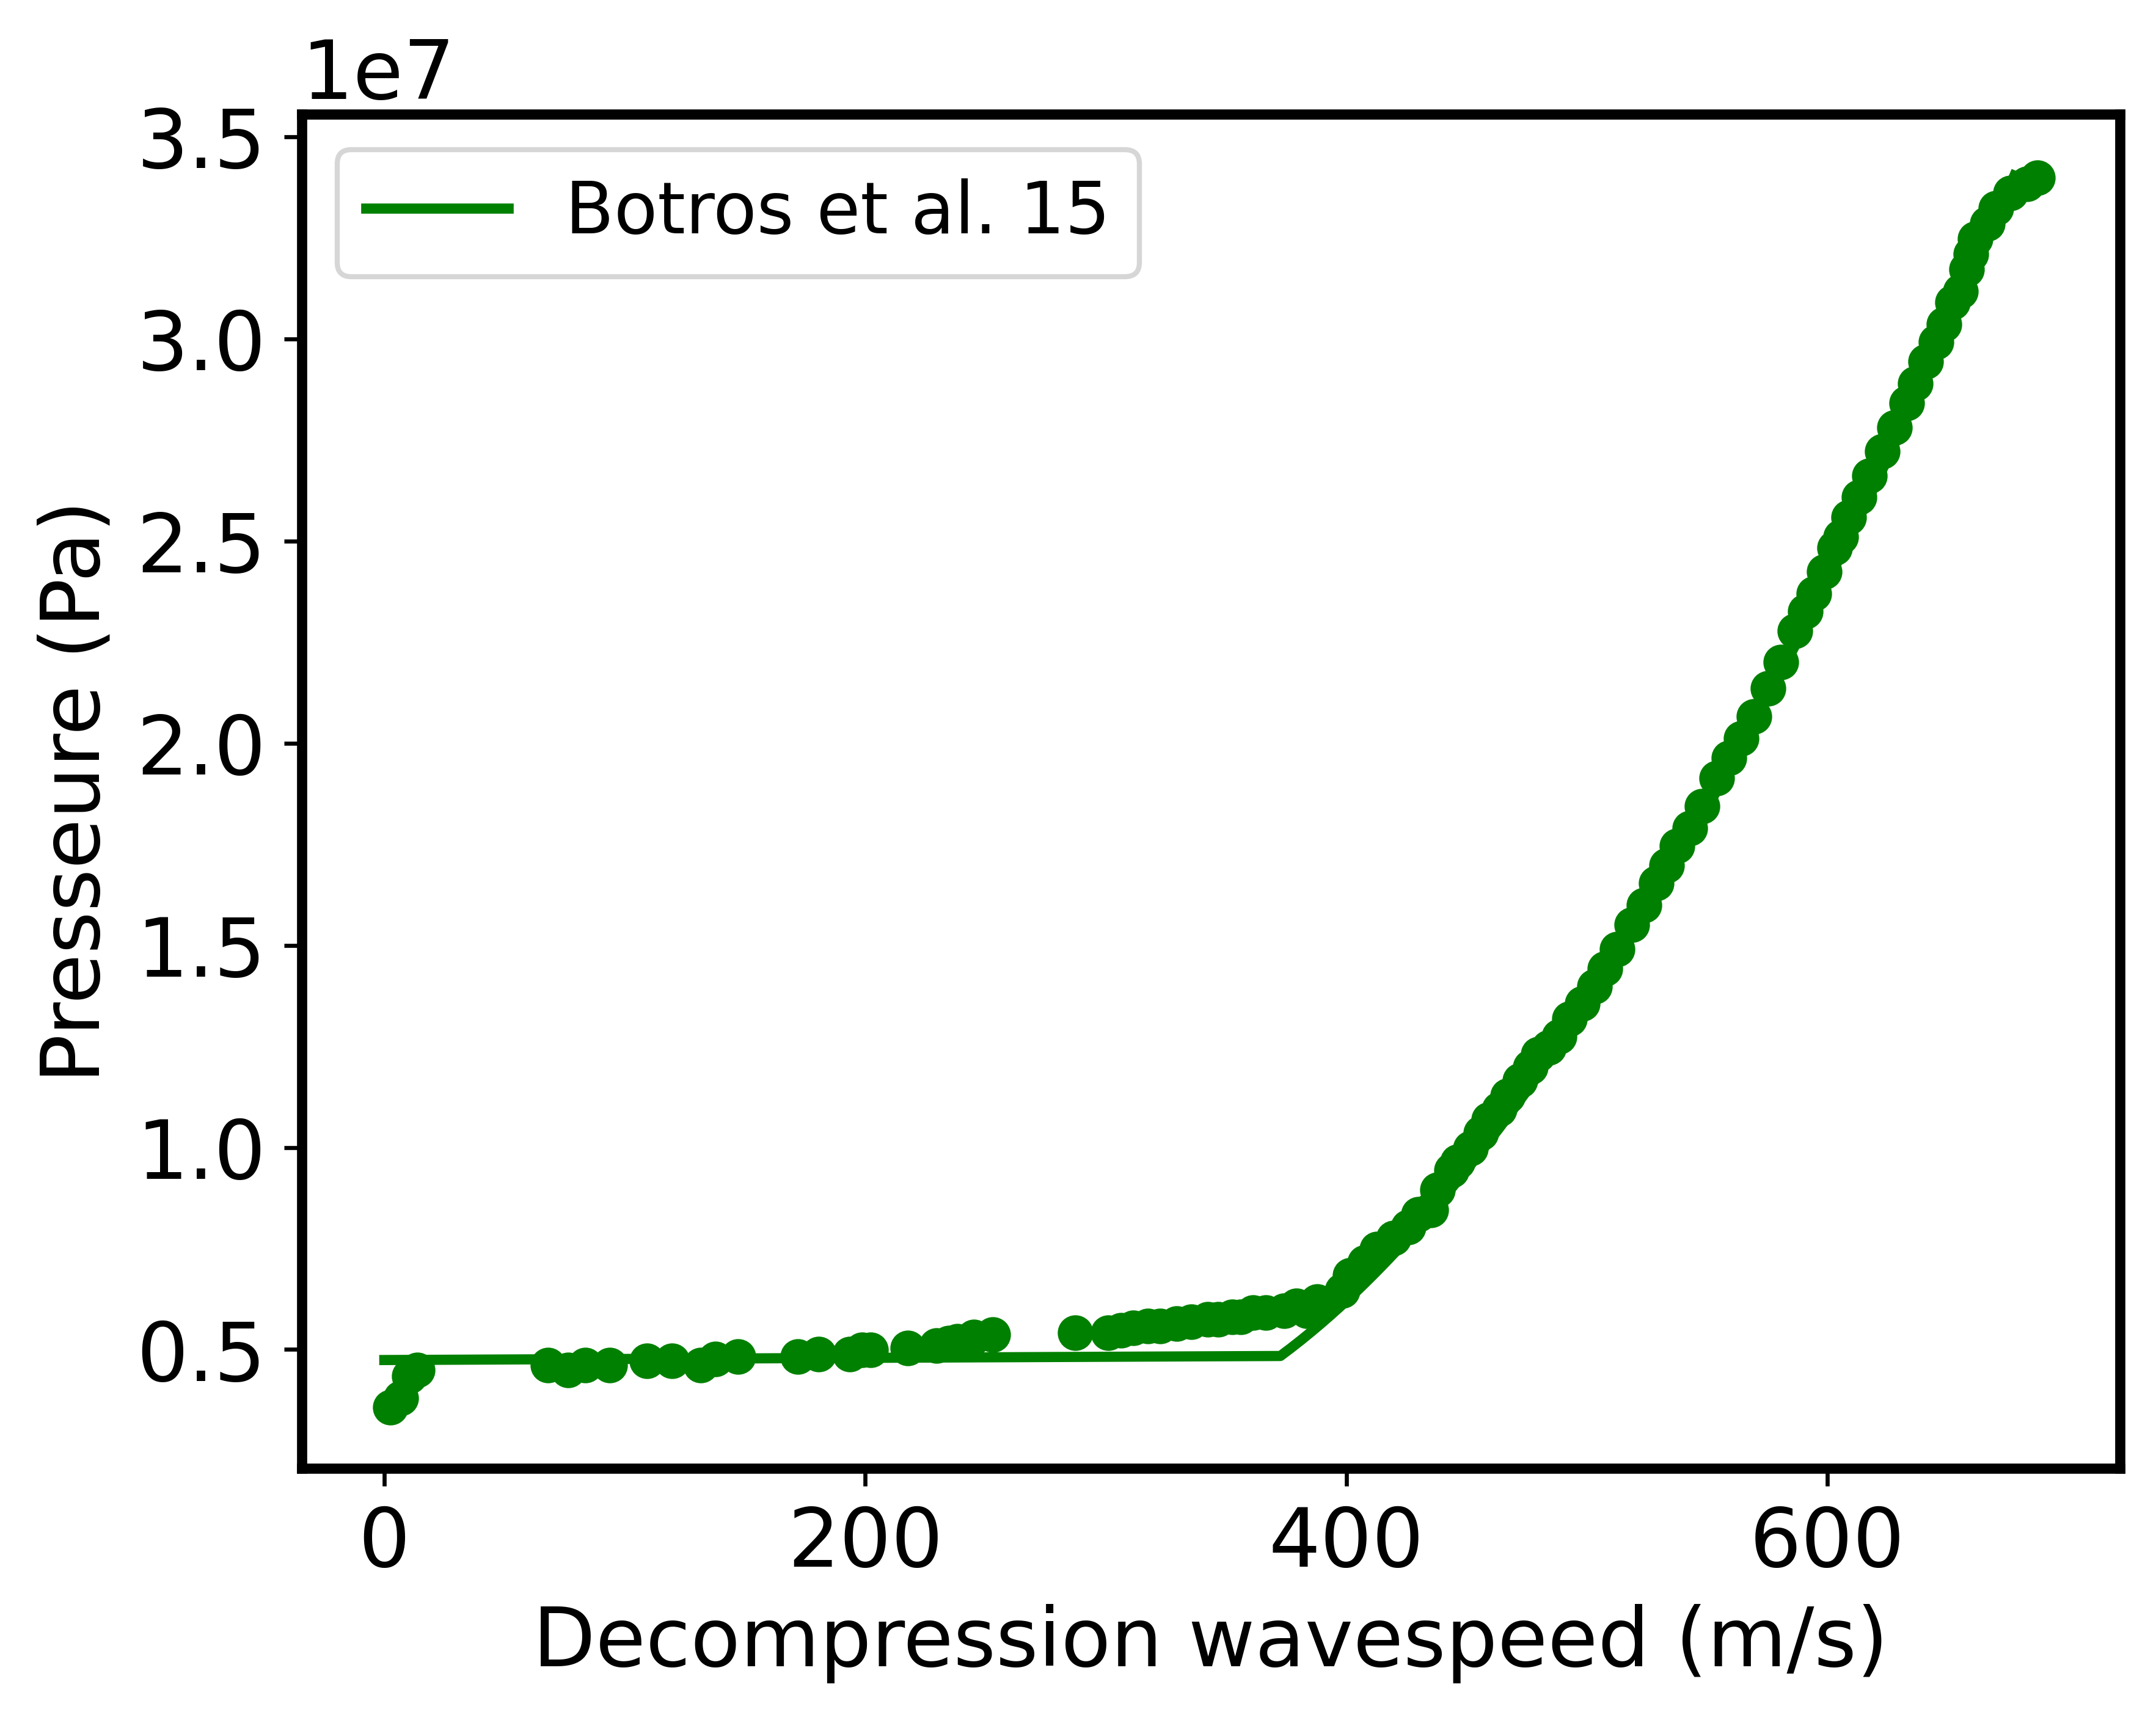
\includegraphics[width=\columnwidth]{./Bilder/pure_3.png}
	\caption{Decompression curve for pure CO$_2$ calculated with the RAMDECOM code and data for experiment 15 from \cite{Botros_pure}.}
	\label{fig:pure_15}
\end{figure}

Generally the following observations are made: First of all, the isentropic decompression path follows a gradual decrease in decompression wave speed as the pressure is reduced. Once the saturation line / two-phase state is reached the decompression wave speed abrubtly drops due to an abrupt drop in the speed of sound, which is seen as a plateau in the pressure.  
Second, it seems that the described decompression wave speed model matches experiments very well for decompression from a supercritical fluid state and this applies to experiments no. 6 \cite{MUNKEJORD2020118560}, 15 \cite{Botros_pure} and 31 \cite{Botros_pure} as seen from Figure \ref{fig:pure_combined} and \ref{fig:pure_15}. Especially the plateau pressure as described previously, is predicted vary well for these cases. Finally, the cases where the decompression starts in the supercritical liquid state and in the gas state are predicted less accurately. This applies to experiments no. 8 \cite{MUNKEJORD2020118560}, 32A \cite{Botros_pure} cf. Figure \ref{fig:pure_combined} and to some extent experiment no. 3 \cite{MUNKEJORD2020118560} cf. Figure \ref{fig:pure_3}. 

In case of experiment no. 3 in Figure \ref{fig:pure_3} the model predicts a slight pressure plateau  at around 3.5 MPa, which is where the theoretical isentropic path intersects the saturation line. However, the experimental data shows a plateau around 2.8 MPa somewhat lower. Munkejord \emph{et al.} \cite{MUNKEJORD2020118560} demonstrated that the experimental data was reasoanbly described is a single phase isentropic path was followed all the way from the initial pressure to the experimental plateau, also supporting a hypothesis that full equilibrium is not established instantaneously and a significant sub-cooling of the gas phase occurs before the first liquid droplets starts to form.  

Experiments 8 and 32A are very similar and in both cases the discrepancy between the predicted plateau pressure and the experimental data have been rationalised by both Botros \emph{et al.} \cite{Botros_pure} and Munkejord \emph{et al.} \cite{MUNKEJORD2020118560} by a very rapid decompression, since the initial pressure is not far from the saturation pressure, in which equilibrium is not due to delayed nucleation. This leads to a measured plateau below the predicted. In both this case and the one for experiment 3 starting from the gas phase it is evident that any non-equilibrium effects be it delayed nucleation or sub-cooled gas, leads to a conservative result from the simple decompression model. 

% Discuss based on p 16 in Munkejord

%\begin{figure*}[!ht]
%\centering
%\mbox{
\includegraphics[width=\textwidth]{./Bilder/SamplePicture.jpg}}
%\caption{A two-column spanning figure.}
%\label{fig:fig_2}
%\end{figure*} 

\subsection{CO$_2$ mixtures}
The calculated decompression curves for the CO$_2$ mixtures in Table \ref{tbl:mix_exp} are shown in Figure \ref{fig:mix_combined} along with the corresponding experimental data from \cite{Botros_mixture}. As seen from the figure experiments no. 4, no. 5, no. 7, and no. 9 are predicted very well by the simple decompression model. The repdictions for these experiments are generally in line with both predictions like the one in the present study using the GERG-2008 \cite{Botros_mixture} equation of state as well as predictions made with GASDECOM \cite{Cosham_GASDECOM}.

\begin{figure}[!ht]
	\centering
	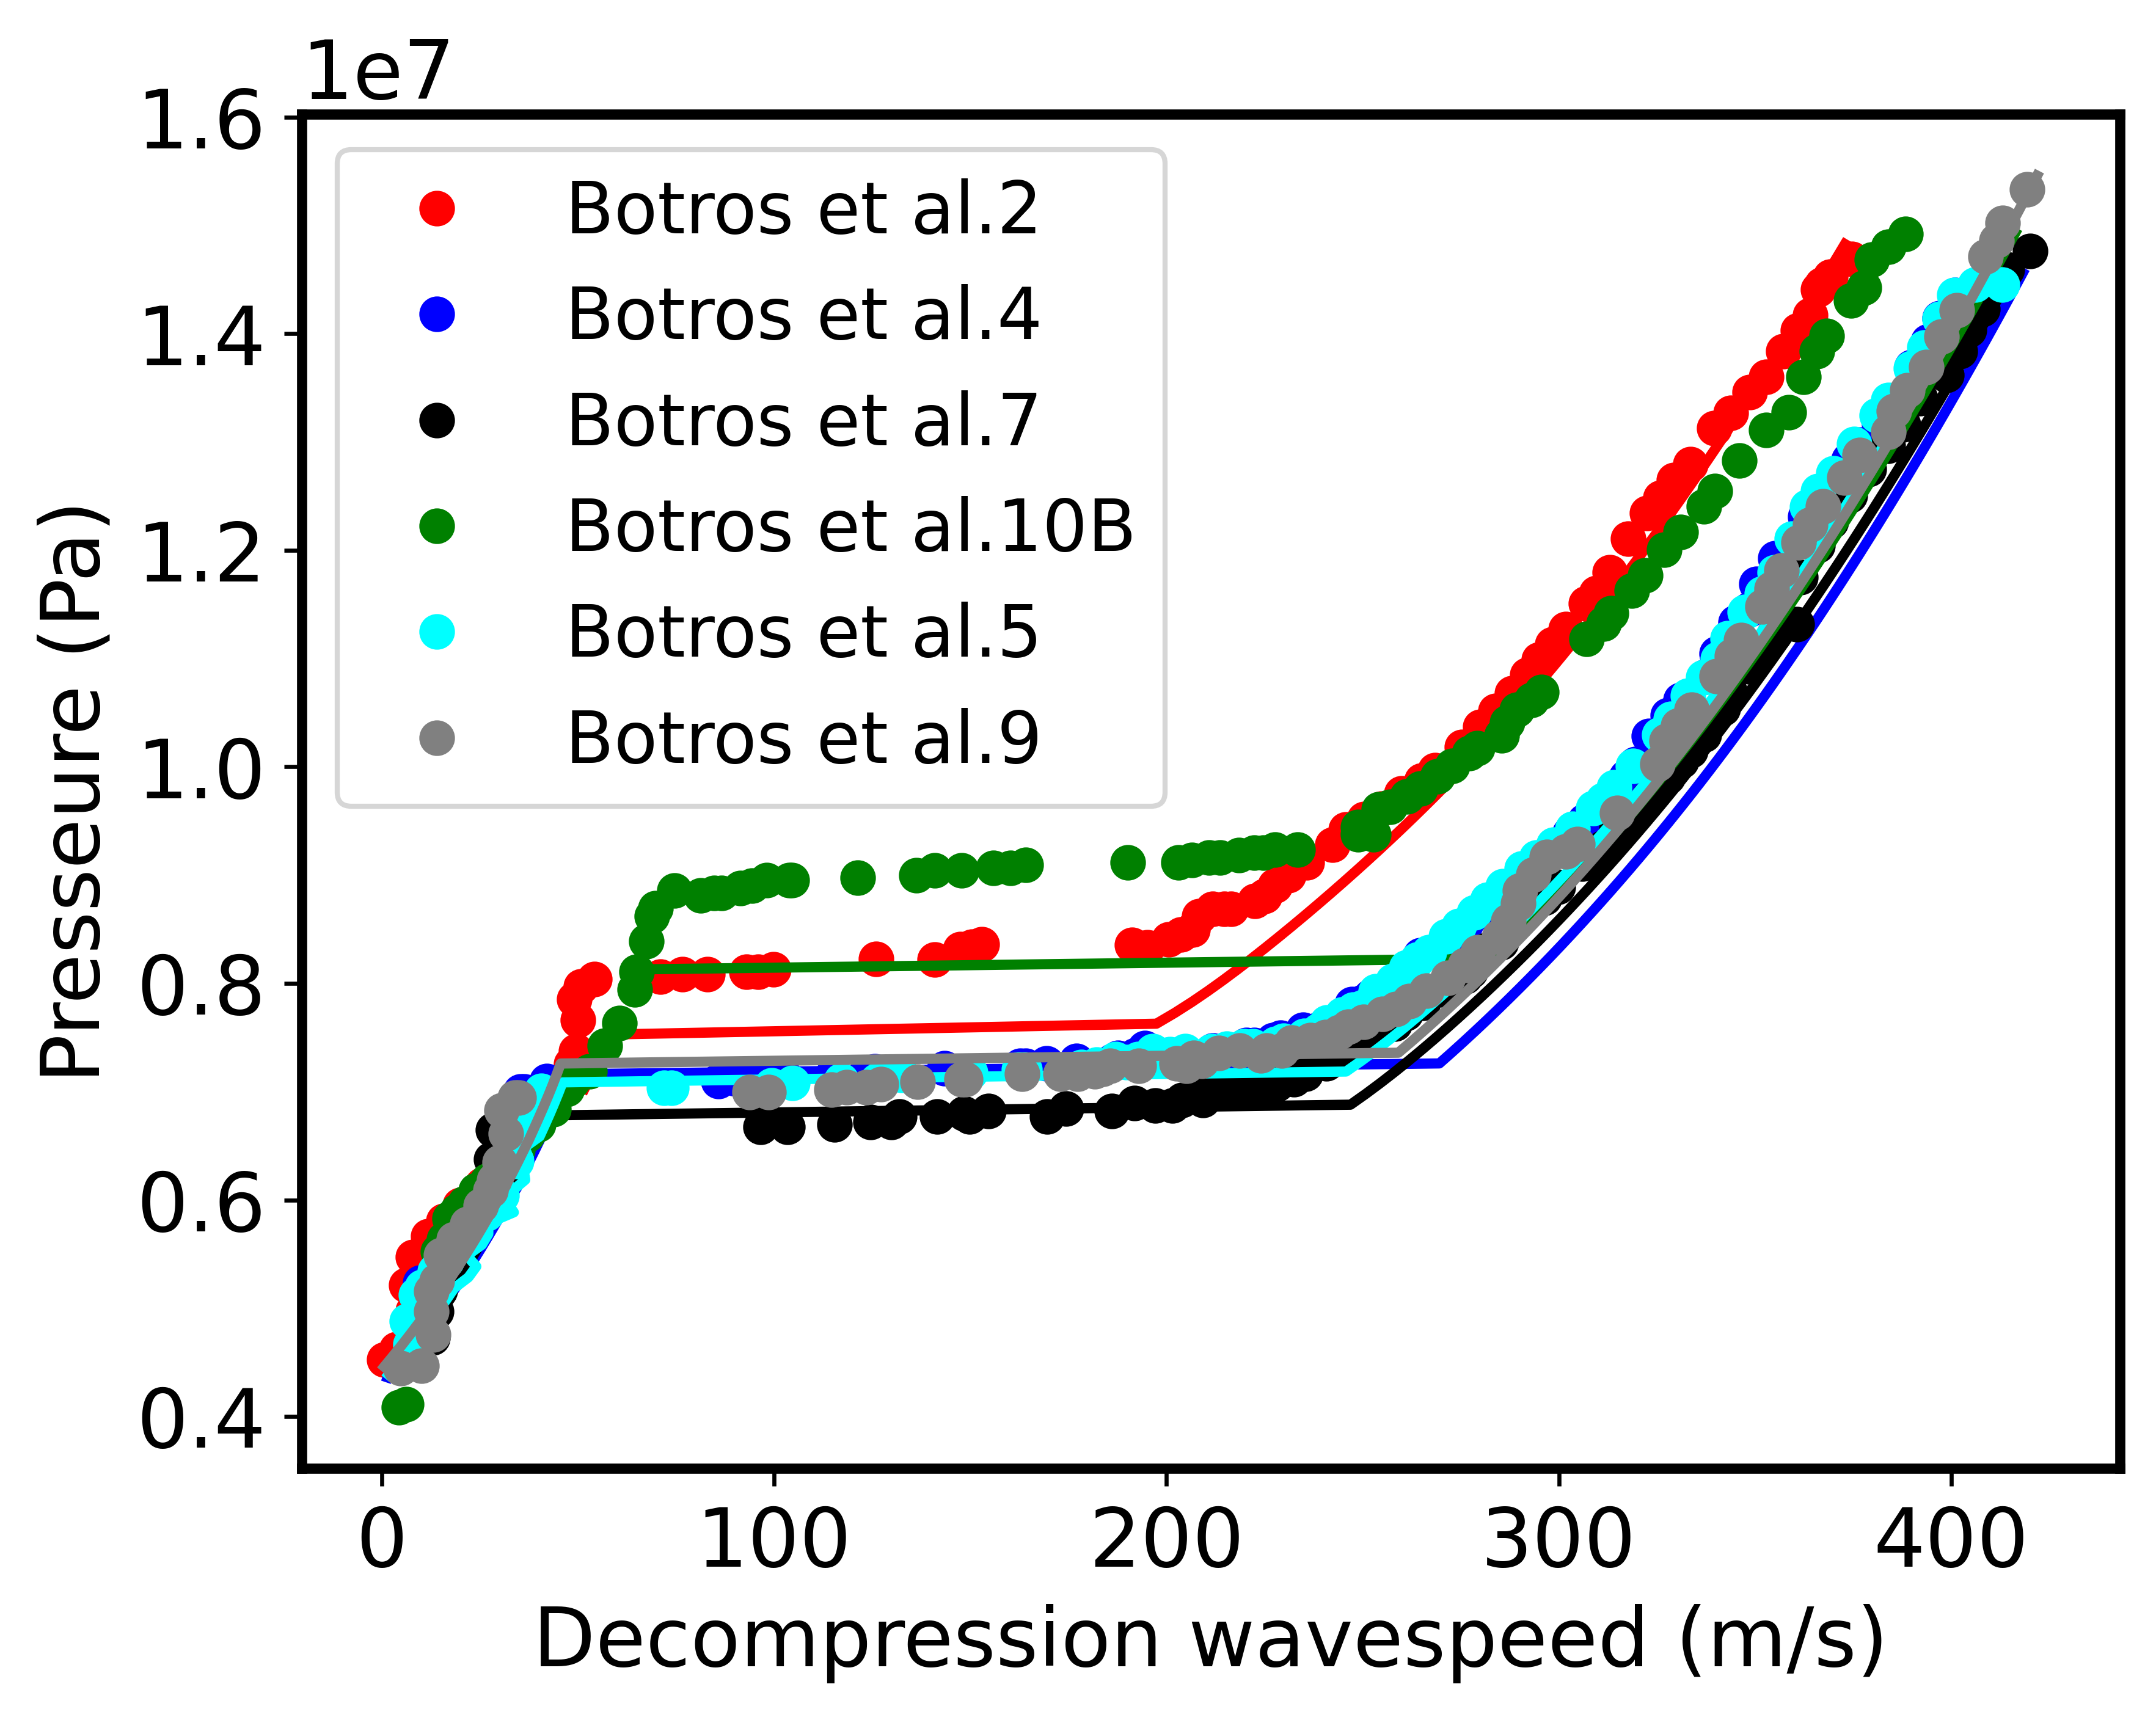
\includegraphics[width=\columnwidth]{./Bilder/mix_combined.png}
	\caption{Decompression curves for rich CO$_2$ mixtures calculated with the RAMDECOM code and experimental data from \cite{Botros_mixture}.}
	\label{fig:mix_combined}
\end{figure}

The main discrepancies between model and experiment are observed for experiment no. 2 and no. 10B, In both cases the simple decompression model under-predicts the plateau pressure. For 10B, which contains a significant amount of hydrogen in a binary mixture, the same model behaviour is observed by Botros \emph{emph} \cite{Botros_mixture}. As observed for the pure CO$_2$ the failure to produce equilibriunm conditions during experiments generally resulted in an over-prediction of the experimentally observed plateau. The fact that the plateau is under-predicted for the H$_2$/CO$_2$ binary mixture could indicate that this is due to a defficiency in the applied equation of state to accurately model the bubble point line in particular. This should be investigated in more detail in future works. 



\Acknowledgement
Acknowledgements come here.



\bibliographystyle{unsrt}
\bibliography{references}


\Appendix
If there is the need for an appendix, this is the right place for it. Again use an unumbered section 
for this purpose, as already used for the introduction. 

%%%%%%%%%%%%%%%%%%%%%%%%%%%%%%%%%%%%%%%%%%%%%%%%%%%%%%%%%%%%%%%%%%%%%%%%%%%%%%%%%%%%%%%%%%%%%%%%%%
\end{document}
